% !TEX encoding = UTF-8 Unicode
%%%%%%%%%%%%%%%%%%%%%%%%%%%%%%%%%%%%%%%%%%%%%%%%%%%%%%%%%%%%%%%%%%%%%%%%%%%%%%%%%%%%%%%%%%%%%%%%%%%%%%% 
%%
%%  This file is asmeconf-template.tex, a LaTeX template to format ASME Conference papers according to
%%  the requirements on ASME's conference web pages, and including hypertext support for the pdf.
%%
%%  This file is version 1.31 dated 2022/07/04
%%  
%%  As of version 1.11, this template defaults to ASME's newer conference guidelines first posted July 2019.
%% 			Those guidelines changed the requested author block formatting to be inline. 
%%			This LaTeX template continues to support the traditional grid format as a package option, [grid].
%%			Nomenclature now follows the abstract. Abstract text is set in italics.
%%
%%  Author: John H. Lienhard V
%%          Department of Mechanical Engineering
%%          Massachusetts Institute of Technology
%%          Cambridge, MA 02139-4307 USA
%%
%%  Class options include:
%%
%%          * Math options from M. Sharpe's newtxmath package: upright integrals [upint]; 
%%          *    [varvw] for a v and w that are better distinguished from Greek nu; and also 
%%          *    [subscriptcorrection, smallerops, varg, frenchmath, varbb, cmbraces, slantedGreek,...] 
%%			* 	 See newtx documentation for descriptions (at CTAN: http://ctan.org, v1.6 or higher is best).
%%
%%          * Options to: 	omit the ASME copyright footer [nofoot]; 
%%			*				use government employee copyright notice [govt];
%%			*				use government contractor copyright notice [contractor]
%%
%%          * An option to use the traditional grid arrangement of author names [grid].  
%%			*	 With this option, line breaks (\\) may be inserted into the address as needed. 
%%			*	 Author names that include commas should be enclosed in braces, e.g., {Joseph L. Smith, Jr.}.  
%%			*	 Authors may be grouped above a single affiliation using braces, e.g., {Henry Tudor, Catherine Parr}.
%%
%%          * An option to balance the heights of columns on the last page [balance]. 
%%          *    This option is NOT compatible with the [lineno] option.
%%
%%          * An option to include line numbers [lineno]. You must *run twice* for proper placement of the line numbers. 
%%			*	 The lineno package does not number titles, footnotes, captions, or tables.
%%          *    This option will disable balancing column height on final page if that option has been invoked.
%%          *    The lineno package won't always number the lines preceding displayed math in a paragraph because
%%          *    paragraph has not ended.  See that package's documentation for macros to address this problem, or
%%          *    just leave a blank line above the displayed equation while you are editing and then remove the 
%%          *    blank line and [lineno] option when you move to your final version.
%%
%%			* Options for PDF/A compliance. [pdf-a] will produce PDF/A-3u compliance with sRGB OutputIntent.
%%			*	 [pdfapart= 1 or 2 or 3] and [pdfaconformance= b or u] can enable levels 1b, 2b, 2u, and 3b.
%%			*    The most recent versions of LaTeX (2021 and later) are moving toward integrated support for pdf-a, 
%%			*    through \DeclareDocumentMetadata{..}. The asmeconf class supports these new features, which can 
%%			*	 replace the aforementioned class options. (An up-to-date LaTeX installation is required to use this.)
%%
%%          * Many options for calligraphic, script, and fraktur fonts from the mathalfa package; the
%%          *    example shown here is: [mathalfa=cal=boondoxo] to use a Boondox font for \mathcal.
%%          *    Some other options for cal are: dutchcal, zapfc, cm (default), euler,...
%%          *    frak (fraktur), bb (blackboard bold), scr (script) may also be chosen this way.
%%			*	 For details, refer to mathalfa documentation (at CTAN: http://ctan.org).
%%
%%          * Option to use superiors font from newtxtext for footnotes [nodefaultsups] and
%%          *    for slightly larger small capitals, [largesc], also from newtxtext.
%%
%%          * An option to allow hyphenation of the typewriter font [hyphenate], from inconsolata package.
%%          *    Hyphenation is normally suppressed for typewriter mode because it is often used for code.
%%			*	 To replace the default variable word spacing by monospacing, use the option [mono].
%%			*	 To get a zero without a slash, use [var0]
%%
%%          * Options (used by the babel package) to include passages in languages other than English (e.g., a translation 
%%			*    of the abstract). Languages are called as options, e.g. [french], [spanish], [greek], [russian], etc. 
%%			*    Language support is greatest when running LuaLaTeX with the [fontspec] option.
%%			*    See Appendix B for details.
%%
%%  The use of commands defined or modified by the asmeconf class is illustrated throughout this file. In particular, 
%%  ASME requires capitalized, sans-serif section headings, and as a result some care is needed when using macros 
%%  in section headings, as also illustrated below.
%%
%%  Use an up-to-date and complete installation of LaTeX, such as TeX Live 2020 or later. Errors may occur with old set-ups.
%%
 %=========================================================
%% 
%% LICENSE: 
%%
%% Copyright (c) 2022 John H. Lienhard
%%
%% Offered under the MIT license: https://ctan.org/license/mit 
%%
%%%%%%%%%%%%%%%%%%%%%%%%%%%%%%%%%%%%%%%%%%%%%%%%%%%%%%%%%%%%%%%%%%%%%%%%%%%%%%%%%%%%%%%%%%%%%%%%%%%%%%% 

%% Class options are described above. Change these options as desired. 
%%		If you are not using the language options, remove them (together with Appendices B and C)
%%	 	Remove the [colorlinks] option before *final* submission to ASME, to get black text for printing,
%%		but keep that option for other uses.
 
\documentclass[balance,upint,subscriptcorrection,varvw,mathalfa=cal=boondoxo,pdf-a,colorlinks,nofoot]{asmeconf}
\usepackage{tikz}
\usetikzlibrary{shapes.geometric, arrows.meta}
\tikzstyle{process} = [rectangle, minimum width=2cm, minimum height=1.3cm, text centered, draw=black]
\tikzstyle{arrow} = [thick,->,>={Stealth[scale=1.1]}]
\usepackage{algorithm, algpseudocode}
\usepackage{siunitx}
\graphicspath{ {../data/} }
%%%%%  pdf metadata  %%%%%%%%%%%%%%%%%%%%%%%%%%%%%%%%%%%%%%%%%%%%%%%%%%%%%%%%%%%%%%%%%%%%%%%%%%%%%%%%%%

\hypersetup{%
	pdfauthor={Yuanhao JIANG},
	pdftitle={Mathematics of Reinforcement Learning with Applications to Quantitative Finance},
	pdfkeywords={Reinforcement Learning,  Artificial Neural Networks},
	pdfsubject={Describe Mathematics of Reinforcement Learning with Applications to Quantitative Finance},
    pdfurl={https://github.com/Yuanhao-JIANG/RL-in-QF},
%	pdflicenseurl={https://ctan.org/pkg/asmeconf},
}

\begin{document}
% Change these fields to the right content for your conference.
% You can comment these out if for some reason you don't want a header.
% Use title case (first letters capitalized), not all capitals
\ConfName{Proceedings of the ASME 2022\linebreak International Mechanical Engineering Congress and Exposition}
\ConfAcronym{IMECE2022}
\ConfDate{October 30--November 3, 2022} % update 
\ConfCity{Columbus, OH} % update 
\PaperNo{IMECE2022-XXXX}

% Units of measure (e.g., cm) and other specialty lowercase terms in the title should be 
%   enclosed in \NoCaseChange{...} to maintain lower case type
%   LaTeX will automatically set the rest of the title in all capital letters.

\title{Mathematics of Reinforcement Learning with Applications to Quantitative Finance}
%\title{Place Title Here: Place Subtitle After Colon} 
 
%   Put author names into the order you want. Use the same order for affiliations.
%   \affil{#} tags the author's affiliation to the address in \SetAffiliation{#}.
%   No space between last name and \affil{#}, separate names with commas.
%
%	For a sole author or a single affiliation for all authors, {#} may be left empty, as \affil{} and \SetAffiliation{} (but not with [grid] option!)
%
%   \CorrespondingAuthor{email} follows that author's affiliation, no spaces.  
%   If multiple corresponding authors, put both email addresses in the same command and place after both authors.
%
%   \JointFirstAuthor, if applicable, follows the affiliation of the relevant authors, no spaces.
\SetAuthors{
	Yuanhao JIANG\affil{1}\CorrespondingAuthor{s2132254@ed.ac.uk}
}

\SetAffiliation{1}{The University of Edinburgh, Edinburgh, UK}
%	To switch from inline author names to gridded names, use the [grid] option.

\maketitle

%%% Change these to your keywords.  Keywords are automatically printed at the end of the abstract.
%%% This command MUST COME BEFORE the end of the abstract.
%%% If you don't want keywords, leave the argument of \keywords{} empty (or use the abstract* environment)
\keywords{Reinforcement Learning, Artificial Neural Networks}

%% Abstract should be 200 words or less
\begin{abstract}
\noindent Abstract goes here.
\end{abstract}

\section{Introduction}
\noindent The object is to use reinforcement learning to solve the following scenario:
a customer arrives with a number of features, we want to promote the customer
with a proper price, such that he is most likely to purchase our product, and 
we also have the highest profit and a better portfolio. 
\vspace{3mm}\newline We can consider this scenario as markov decision process,
with the current state being the current customer features and current 
portfolio. At each time step, the agent promote a price according to the 
current customer features and the current portfolio, after that the customer 
resopnse to the action. The reward is then given besed on the customer 
response and the portfolio. Then the portfolio updates and a new customer 
arrives.

\section{Reinforcement Learning}
\noindent The reinforcement learning method we want to use is based on the Markov 
decision process (MDP), as illustrated in Figure~\ref{fig:MDP-illustration}.
\begin{figure}
    \centering
    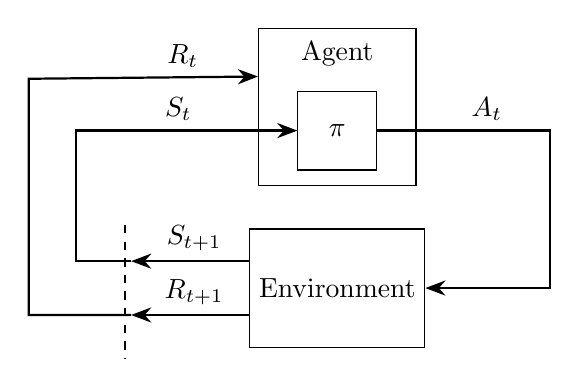
\begin{tikzpicture}
        \node (agent) [process, minimum width=2cm, minimum height=2cm,
            label={[anchor=north,inner sep=5pt]north:Agent}]{};
        \node (pi) [process, left of=agent, minimum width=1cm, 
            minimum height=1cm,xshift=1cm, yshift=-0.3cm] {\(\pi\)};
        \node (env) [process, minimum height=1.5cm, below of=pi, yshift=-1cm] 
            {Environment};

        \draw [arrow] (env.163) -- ++(-1.5,0) node[anchor=south, xshift=0.8cm]
            {\(S_{t+1}\)} coordinate(a1);
        \draw [arrow] (a1) -- ++(-0.7,0) |- node[anchor=south, xshift=1.3cm] 
            {\(S_t\)} (pi);
        \draw [arrow] (env.197) -- ++(-1.5,0) node[anchor=south, xshift=0.8cm]
            {\(R_{t+1}\)} coordinate(a2);
        \draw [arrow] (a2) -- ++(-1.3,0) -- ++(0,3) 
            -- node[anchor=south, xshift=0.5cm] {\(R_t\)} (agent.159);
        \draw [arrow] (pi) -- ++(2.7,0) node[anchor=south, xshift=-0.8cm] 
            {\(A_t\)} |- (env);
        \draw [dashed,thick] (-2.7,-1.5) -- (-2.7, -3.2);
    \end{tikzpicture}
    \caption{MDP Illustration}
    \label{fig:MDP-illustration}
\end{figure}
\noindent However, in RL, the agent is not told which actions to take, but 
instead must discover which actions yield the most reward by trying them. Our 
goal at each time step is to find a policy \(\pi\) to maximize the expected 
reward alonge the process afterwards, which is given by the value function
\[V(s)=\mathbb{E}\left[\sum_{i=0}^{\infty} \gamma^i R_{t+i+1}\;\middle|\; 
S_t=s\right]\]
To achieve this, we need to evaluate the current policy, and improve it 
accordingly.

\subsection{Policy Evaluation}
\noindent We want to evaluate the value function under a given policy \(\pi\).
According to Bellman equation,
\[v_\pi(s)=\mathbb{E}_\pi\left[R_{t+1}+\gamma v_\pi(S_{t+1})\;\middle|\;
S_t=s\right]\]
We can use it to iteratively compute \(v_\pi\). The iteratively update is
\[v_{k+1}(s)=\mathbb{E}_\pi\left[R_{t+1}+\gamma v_k(S_{t+1})\;\middle|\;
S_t=s\right]\]
which is proven that it will converge to the true value given any initial value 
function.

\subsection{Policy Improvement}
\noindent Now we have the evaluated value function for the policy, we want to 
improve it accordingly. To do this, we introduce the q-function under 
policy \(\pi\)
\[q_\pi(s, a) = \mathbb{E}\left[R_{t+1} + \gamma v_\pi(S_{t+1})\;\middle|\;
S_t=s, A_t=a\right]\]
The policy improvement theorem says that, let \(\pi\) and \(\pi'\) be any pair
of policy, for all \(s\) we have
\[q_\pi(s, \pi'(s))\geq v_\pi(s) \:\Rightarrow\: v_{\pi'}(s) \geq v_\pi(s)\]
Now we can improve the policy by
\[\pi'(s)=\underset{a}{\text{argmax}}\:q_\pi(s,a)\]
for all \(s\).

\subsection{Policy Iteration}
\noindent By iteratively applying policy evaluation and policy improvement, we
can obtain a sequence of monotonically improving policies and value functions:
\[\pi_0 \overset{E}{\longrightarrow} v_{\pi_0} \overset{I}{\longrightarrow}
\pi_1 \overset{E}{\longrightarrow} v_{\pi_1} \overset{I}{\longrightarrow}
\dots \overset{I}{\longrightarrow} \pi_* \overset{E}{\longrightarrow} v_*\]
where \(\overset{E}{\longrightarrow}\) denotes a policy evaluation and
\(\overset{I}{\longrightarrow}\) denotes a policy improvement. This way of 
finding an optimal policy is called policy iteration.

\subsection{Value Iteration}
\noindent One drawback to policy iteration is that each of its iterations 
involves policy evaluation, which itself is a protracted iterative computation
requiring multiple sweeps through the state set.
\vspace{3mm}\newline We now truncate the policy evaluation such that it is
stopped after just one sweep (one update of each state):
\begin{align*}
    v_{k+1}(s)&=\underset{a}{\text{max}}\:q(s, a)\\
              &=\underset{a}{\text{max}}\:\mathbb{E}\left[
          R_{t+1}+\gamma v_k(S_{t+1})\;\middle|\;S_t=s, A_t=a\right]
\end{align*}
We keep iterate until \(v\) converges (to \(v_*\)), then we record the last
policy \(\pi(s) = \underset{a}{\text{argmax}}\:q(s, a)\).

\subsection{Generalized Policy Iteration}
\noindent As long as both processes, policy evaluation and policy improvement,
continue to update all states, the ultimate result is typically the 
same --- converge to the optimal value function and an optimal policy.
\vspace{3mm}\newline Generalized policy iteration (GPI) is used to refer to the
general idea of letting policy evaluation and policy improvement interact,
independent of the granularity of the two processes (instead of letting each
complete before the other begins).

\subsection{Temporal-Difference Learning}
\noindent When we don't have the complete model of the environment, we need to 
estimate the value function from only experience. There are two methods to do 
so: Monte Carlo Methods and Temporal-Difference. We will use 
Temporal-Difference method in this project.
\vspace{3mm}\newline To estimate \(v_\pi(S_t)\) using only the experience, we 
take the average on all experienced trajectory' values. Temporal-Difference
method uses \(G_i = [R_{t+1}]_i+\gamma [v_\pi(S_{t+1})]_i\) to estimate the 
value of the \(i\)th trajectory starting at \(S_t\), with \(v_\pi\) being the 
estimated value function at the \(i\)th time \(S_t\) is visitied, which can be 
initialized to anything at start. Now we have the incremental formula to update
our value function:
\begin{align*}
    &[v_\pi(S_t)]_{k+1} \\
    =\:& \frac{1}{k}\sum_{i=1}^{k} G_i\\
    =\:& \frac{1}{k}\left(G_k + \sum_{i=1}^{k-1} G_i\right)\\
    =\:& \frac{1}{k}\left(G_k + (k-1)[v_\pi(S_t)]_{k}\right)\\
    =\:& [v_\pi(S_t)]_k + \frac{1}{k}(G_k-[v_\pi(S_t)]_k)\\
    =\:& [v_\pi(S_t)]_k + \frac{1}{k}
    ([R_{t+1}]_k+\gamma [v_\pi(S_{t+1})]_k-[v_\pi(S_t)]_k)
\end{align*}
To simplify:
\[v_\pi(S_t)\longleftarrow v_\pi(S_t)+\alpha
[R_{t+1}+\gamma v_\pi(S_{t+1})-v_\pi(S_t)]\]
with \(\alpha\) being the stepsize. And this also applies to the q function:
\begin{multline*}
    q_\pi(S_t, A_t)\longleftarrow q_\pi(S_t, A_t)\\
    +\alpha[R_{t+1}+\gamma q_\pi(S_{t+1}, A_{t+1})-q_\pi(S_t, A_t)]
\end{multline*}

\subsection{Policy Gradient Methods}
\noindent When the state space is arbitrarily large, we cannot find an optimal 
policy or the optimal value function given the limited resources and time. 
Instead of keeping track of the value and the action(s) to select for each 
state (tabular methods), we can use parameterized functions, for example, 
artificial neural networks (ANNs), to approximate the value function and the 
policy function.
\vspace{3mm}\newline Previously methods learned the values of actions and then
select actions based on their estimated action values (q function). Now we
consider methods that instead learn a parameterized policy that select actions
without consulting a value function. A value function may still be used to
learn the policy parameter, but is not required for action selection.
\vspace{3mm}\newline We use \(\bm{\theta}\) and \(\bm{w}\) to denotes the
policy's parameter vector and value function's weight vector, respectively.
Then we have our policy \(\pi\left(a\;\middle|\;s, \bm{\theta}\right)
=\text{Pr}\left\{A_t=a\;\middle|\;S_t=s, \bm{\theta}_t=\bm{\theta}\right\}\) and
value function \(v_\pi(s, \bm{w})\). We also define the scalar performance
measure (objective) to be
\[J(\bm{\theta})=\begin{cases}
    \ v_{\pi_{\bm{\theta}}}(s_0); &\text{episodic case}\\
    \ \lim_{t \to \infty} \mathbb{E}
    \left[R_t\;\middle|\;S_0,A_{0:t-1}\sim\pi\right];
                                  & \text{continuing case}
\end{cases}\]
Policy gradient methods seeks to maximize this performance measure, so their
updates approximate gradient ascent in \(J\):
\[\bm{\theta}_{t+1}=\bm{\theta}_t+\alpha\widehat{\nabla J(\bm{\theta}_t)}\]
where \(\widehat{\nabla J(\bm{\theta}_t)}\) is a stochastic estimate whose
expection approximates the gradient of the performance measure w.r.t
\(\bm{\theta}_t\).

\subsubsection{The Policy Gradient Theorem}
The policy gradient theorem says
\[\nabla J(\bm{\theta})\propto \sum_{s} \mu(s)
\sum_{a} q_\pi(s,a)\nabla\pi\left(a\middle|s, \bm{\theta}\right)\]
where \(\mu\) is the stationary distribution of the state. Thus we can derive
\begin{align*}
    \nabla J(\bm{\theta})
    &\propto \sum_{s} \mu(s)
    \sum_{a} q_\pi(s,a)\nabla\pi\left(a\middle|s, \bm{\theta}\right)\\
    &= \mathbb{E}_\pi\left[\sum_{a} q_\pi(S_t,a)
    \nabla\pi\left(a\middle|S_t, \bm{\theta}\right)\right]\\
    &= \mathbb{E}_\pi\left[\sum_{a} \pi\left(a\middle|S_t, \bm{\theta}\right)
        q_\pi(S_t,a)\frac{\nabla\pi\left(a\middle|S_t, \bm{\theta}\right)}
        {\pi\left(a\middle|S_t, \bm{\theta}\right)}\right]\\
    &=\mathbb{E}_\pi\left[q_\pi(S_t,A_t)
        \frac{\nabla\pi\left(A_t\middle|S_t, \bm{\theta}\right)}
        {\pi\left(A_t\middle|S_t, \bm{\theta}\right)}\right]
\end{align*}
The policy gradient theorem can be generalized to include a comparison of the
action value to an arbitrary baseline \(b(s)\):
\[\nabla J(\bm{\theta})\propto \sum_{s} \mu(s) \sum_{a}
    \Bigl(q_\pi(s,a)-b(s)\Bigr)\nabla\pi\left(a\middle|s, \bm{\theta}\right)\]
with the same derivation we have
\[\nabla J(\bm{\theta})\propto\mathbb{E}_\pi\left[
        \Bigl(q_\pi(S_t,A_t)-b(S_t)\Big)
        \frac{\nabla\pi\left(A_t\middle|S_t, \bm{\theta}\right)}
{\pi\left(A_t\middle|S_t, \bm{\theta}\right)}\right]\]
And the discounted version of above is:
\[\nabla J(\bm{\theta})\propto\mathbb{E}_\pi\left[
        \gamma^{t}\Bigl(q_\pi(S_t,A_t)-b(S_t)\Big)
        \frac{\nabla\pi\left(A_t\middle|S_t, \bm{\theta}\right)}
{\pi\left(A_t\middle|S_t, \bm{\theta}\right)}\right]\]
One natural choice for baseline is an estimate of the state value,
\(\hat{v}(S_t, \bm{w})\), where \(\bm{w}\) is the weight vector to be learned.

\subsubsection{Actor-Critic Methods}
Recall the TD method, we make use of 
\(q_\pi(s,a)=\mathbb{E}\left[R_{t+1}+\gamma v_\pi(S_{t+1})\;\middle|\;
S_t=s, A_t=a\right]\), by taking one sample estimate, and choosing
\(\hat{v}(S_t, \bm{w})\) as baseline, we have
\[\nabla J(\bm{\theta})\propto\mathbb{E}_\pi\left[
        \Bigl(R_{t+1}+\gamma \hat{v}(S_{t+1}, \bm{w})-\hat{v}(S_t, \bm{w})\Big)
        \frac{\nabla\pi\left(A_t\middle|S_t, \bm{\theta}\right)}
{\pi\left(A_t\middle|S_t, \bm{\theta}\right)}\right]\]
Again, by taking one sample estimate we have the update formula for 
\(\bm{\theta}\):
\begin{align*}
    \bm{\theta}_{t+1}
    &=\bm{\theta}_t + \alpha_{\bm{\theta}}
    \Bigl(R_{t+1}+\gamma \hat{v}(S_{t+1}, \bm{w})-\hat{v}(S_t, \bm{w})\Big)
    \frac{\nabla\pi\left(A_t\middle|S_t, \bm{\theta}_t\right)}
    {\pi\left(A_t\middle|S_t, \bm{\theta}_t\right)}\\
    &=\bm{\theta}_t+\alpha_{\bm{\theta}}\delta_t
    \nabla\ln{\pi\left(A_t\middle|S_t, \bm{\theta}_t\right)}
\end{align*}
As for the weight vector \(\bm{w}\) for the estimated value function, at each 
time step \(t\), we want to update it by minimizing the squared error,
\(\bigl[v_\pi(S_t)-\hat{v}(S_t, \bm{w}_t)\bigr]^2\):
\begin{align*}
    \bm{w}_{t+1} 
    &= \bm{w}_t - 
    \alpha_{\bm{w}}'\nabla \Bigl[v_\pi(S_t)-\hat{v}(S_t, \bm{w}_t)\Bigr]^2\\
    &= \bm{w}_t - \alpha_{\bm{w}}\Bigl(v_\pi(S_t)-\hat{v}(S_t, \bm{w}_t)
    \Bigr)\nabla \hat{v}(S_t, \bm{w}_t)
\end{align*}
where \(v_\pi\) is the true value function. Again, since \(v_\pi(s)=
\mathbb{E}\left[R_{t+1}+\gamma v_\pi(S_{t+1})\;\middle|\;S_t=s\right]\), we
take one sample estimate, which gives us the update formula for \(\bm{w}\):
\begin{align*}
    \bm{w}_{t+1} 
    &= \bm{w}_t - \alpha_{\bm{w}}
    \Bigl(R_{t+1}+\gamma\hat{v}(S_{t+1},\bm{w})-\hat{v}(S_t, \bm{w}_t)
    \Bigr)\nabla \hat{v}(S_t, \bm{w}_t)\\
    &=\bm{w}_t - \alpha_{\bm{w}}\delta_t\nabla \hat{v}(S_t, \bm{w}_t)
\end{align*}
The actor-critic method is based on the above updates formulas, details are
shown in Algorithm \ref{algorithm:actor-critic}.
\begin{algorithm}
    \caption{Actor-Critic\label{algorithm:actor-critic}}
    \begin{algorithmic}[1]
        \State Input: a differentiable policy parameterization 
        \(\pi\left(a\middle|s, \bm{\theta}\right)\)
        \State Input: a differentiable state-value function parameterization
        \(\hat{v}(s,\bm{w})\)
        \State Step sizes \(\alpha_{\bm{\theta}}>0\), \(\alpha_{\bm{w}}>0\)
        \State \(\bm{\theta} \gets \bm{0}\), \(\bm{w} \gets \bm{0}\)
        \Loop \hspace{0.3mm} (for each episode)
        \State Initialize \(S\) (first state of the episode)
        \Loop \hspace{0.3mm} (for each time step \(i\))
        \State \(A\sim\pi\left(\cdot\middle|S, \bm{\theta}\right)\)
        \State Take action \(A\), observe \(S'\), \(R\)
        \State \(\delta \gets R + \gamma\hat{v}(S',\bm{w})-\hat{v}(S,\bm{w})\)
        \State \(\bm{w} \gets \bm{w} + 
        \alpha_{\bm{w}} \delta\nabla\hat{v}(S,\bm{w})\)
        \State \(\bm{\theta} \gets \bm{\theta} 
        + \alpha_{\bm{\theta}}\gamma^{i}\delta
        \nabla\ln{\pi\left(A\middle|S, \bm{\theta}\right)}\)
        \State \(S \gets S'\)
        \EndLoop
        \EndLoop
    \end{algorithmic}
\end{algorithm}

\section{Build the Environment}
\noindent The environment does the following things:
\begin{enumerate}
    \item record the current state that can be queried anytime
    \item when an action, i.e. a price, is given according to the current 
        state, it outputs the reward, and goes to next state
\end{enumerate}
At each time step, the state consists of a randomly generated customer's 
features and the current portfolio. After the agent performs an action, i.e.
promotes a price to the customer, the reward is then computed based on the 
profit on this customer and the portfolio up to now.

\subsection{Customer Features}
\noindent A customer's features is represented by an array (or vector), denoted 
by \(x\) with 16 entries with each generated randomly from a distribution, 
including normal distribution, binomial distribution, and so on. For example, 
a feature vector \(x\) is described as Table \ref{tab:1}
\begin{table*}
    \caption[Table]{Customer Feature Vector Description\label{tab:1}}
    \centering
    \begin{tabular}{c|c|c|c|c|c|c|c}
        gender & age & car cost & miles & brand & random feature 0 & random 
        feature 1 & \dots\\
        \hline
        1.0 & 42.723 & 94032.096 & 30086.311 & 29.264 & 8.0 & 68.740 & \dots
    \end{tabular}
\end{table*}

\noindent After a price, denoted by \(c\), is promoted to a customer, the 
customer will give a resopnse, denoted by \(r\), which is 0 if he does not buy
the product, and 1 otherwise. And the profit we have for that customer, 
denoted by pf, can be computed by
\[\text{pf} = r*\left(c - g(x)\right)\]
where \(g(x)\) is the cost on that customer.

\subsection{Resopnse}
\noindent The resopnse is generated by a generalized linear model, whose input 
is a vector of a customer features vector \(x\) appended with a price \(c\), 
i.e. \(r=glm(x[0], \dots, x[15], c)\).
\vspace{3mm}\newline The GLM used in the project is fitted using a randomly
generated data set with each observation is a customer's features followed by 
a price, then followed by a resopnse, as illustrated by Table \ref{tab:2}.
\begin{table*}
    \caption[Table]{Customer Feature Vector Description\label{tab:2}}
    \centering
    \begin{tabular}{c|c|c|c|c|c}
        & customer feature 0 & \dots & customer feature 15 & price & resopnse\\
        \hline
        1 & 1.0 & \dots & 2.0 & 1109.504 & 1.0\\
        \hline
        2 & 0.0 & \dots & 1.0 & 665.8 & 0.0\\
        \hline
        \dots & \dots & \dots & \dots & \dots & \dots
    \end{tabular}
\end{table*}

\vspace{3mm}\noindent And the link function for the GLM is chosen to be the logistic function.

\subsection{State}
\noindent The state at start of each time step is the feature vector of the 
new customer to promote (might be modified a bit), appended by the portfolio, 
which is also a data vector consists of the following entries:
\begin{itemize}
    \item average profit over all customers so far, expect for the new customer
        at current time step, denoted by avg\_pf (initialized to \(0\)), 
        which is computed by
        \[\text{avg\_pf}_t = \frac{1}{t}\sum_{i=0}^{t-1} \text{pf}_i, \:t>0\]
    \item the portion of the buyers over all customers, expect for the new one,
        denoted by p (initialized to 0), which is computed by
        \[\text{p}_t=\frac{1}{t}\sum_{i=0}^{t-1} r_i, \:t>0\]
    \item the variance of the portion of buyers in their categories, denoted 
        by var: we divide customers (expect for the new one at current time 
        step) into 4 categories, according to their features, and for each 
        category, we compute the portion of the customers who buy our product,
        denoted by \(\text{pt}_i\) with \(i=1, 2, 3, 4\), then we compute the 
        variance of the 4 portions:
        \[\text{var}=\text{Var}(\text{pt})=\frac{\sum_{i=1}^{4} 
        \left(\text{pt}_i-\bar{\text{pt}}\right)^2}{3}\]
        Later we use this to compute reward to 
        make sure the agent will promote to all types of customers instead of 
        only focusing on one type. Note that \(\text{var}\leq1\).
\end{itemize}
Thus, the state \(s\), or \(s_t\), end up with the form
\[s_t=
(x'_t[0],\:\dots,\:x'_t[-1],\:\text{avg\_pf}_t,\:\text{p}_t, \:\text{var}_t)\]
where \(x'_t\) is the modified \(x_t\), including preprocess
of converting some categorical data to meaningful data to the model.

\subsection{Reward}
\noindent The reward at each time step \(t\), after the price \(c_t\) is 
promoted to the customer \(x_t\), denoted by \(R_t\), is calculated by
\[R_t = \text{pf}_t\left(1-h(\text{var}_t)\right)\]
where \(h\) is a function that indicates how much we care about the variance,
i.e. how important it is to try to promote to customers of all categories. In
this project I choose \(h\) to be such that 
\(h(\text{var}) = \sqrt{\text{var}}/2\).

\section{Build the model}
\noindent With the environment well built, we now build the model for our 
policy and the value function. In this project we use artificial neuro networks
(ANNs) as the parameterized policy and value function, each with three linear 
layers, and with the ReLU function as the activation function. And the input 
of both function is the state, as illustrated in Figure~\ref{fig:ANN}.
\begin{figure*}
    \centering
    \[S_t\rightarrow\underset{\text{ANN for value function}}{
            \boxed{
                \underset{n(S)\rightarrow 128}{\text{Linear}}
                \rightarrow\text{ReLU}
                \rightarrow\underset{128\rightarrow 128}{\text{Linear}}
                \rightarrow\text{ReLU}
                \rightarrow\underset{128\rightarrow 1}{\text{Linear}}
            }
    }\rightarrow v_t\]
    \[S_t\rightarrow\underset{\text{ANN for policy function}}{
            \boxed{
                \underset{n(S)\rightarrow 128}{\text{Linear}}
                \rightarrow\text{ReLU}
                \rightarrow\underset{128\rightarrow 128}{\text{Linear}}
                \rightarrow\text{ReLU}
                \rightarrow\underset{128\rightarrow n(A)}{\text{Linear}}
                \rightarrow\underset{(0.1, \: 0.1)}{\text{Threshold}}
            }
    }\rightarrow \pi_t\rightarrow c_t\]
    \caption{ANN model for policy and value function\label{fig:ANN}}
\end{figure*}
where \(n(S)\) denotes the vector length of the state and \(n(A)\) denotes 
the number of actions. 
\vspace{3mm}\newline We generate the policy distribution by scoring each 
action. E.g. denoted the policy function output by \(y\), then the probability 
of choosing action \(i\) (\(i=0, 1, ..., n(A) - 1\)) is computed by 
\[P(i)=\frac{y_i}{\sum_{j=0}^{n(A)-1} y_j}\]
Note that we add a Threshold layer at the end of policy 
function, which is defined by 
\[\text{Threshold}(0.1, 0.1)=\text{max}(0.1, x)\]
which makes sure that 
\begin{enumerate}
    \item the probabilities are valid (no negative values, greater score 
        results in greater probability);
    \item all actions have the probability to be chosen at early stage, which 
        is beneficial for training since it increase the exploration for 
        different actions.
\end{enumerate}

\section{RL with Actor-Critic}
\noindent In this project, we consider the episodic learning procedure, where 
each episode has finite time steps, \(T\), to be specified as a constant, and 
we will also reset the environment at the start of each episode.

\subsection{The Algorithm}
\noindent Algorithm \ref{algorithm:actor-critic-fin} uses RL with actor-critic 
method, and with the help of what we have built in previous sections, to solve 
the problem.
\begin{algorithm}
    \caption{Actor-Critic for financial problem
        \label{algorithm:actor-critic-fin}
    }
    \begin{algorithmic}[1]
        \State Initialize ANN policy parameterization
        \(\pi\left(c\middle|s, \bm{\theta}\right)\), with any \(\bm{\theta}\)
        \State Initialize ANN state-value function parameterization
        \(\hat{v}(s,\bm{w})\) with any \(\bm{w}\).
        \State Step sizes \(\alpha_{\bm{\theta}}>0\), \(\alpha_{\bm{w}}>0\)
        \Loop \hspace{0.3mm} (for each episode)
        \State Reset the environment
        \State Generate an \(x\) (first customer of the episode)
        \State Initialize \(S\) (first state of the episode)
        \For{\(t=0, 1, ..., T\)}
        \State \(c\sim\pi\left(\cdot\middle|S, \bm{\theta}\right)\)
        \State Take action \(c\), observe \(S'\), \(R\) from environment
        \State \(\delta \gets R + \gamma\hat{v}(S',\bm{w})-\hat{v}(S,\bm{w})\)
        \State \(\bm{w} \gets \bm{w} +
        \alpha_{\bm{w}} \delta\nabla\hat{v}(S,\bm{w})\)
        \State \(\bm{\theta} \gets \bm{\theta}
        + \alpha_{\bm{\theta}}\gamma^{t}\delta
        \nabla\ln{\pi\left(A\middle|S, \bm{\theta}\right)}\)
        \State \(S \gets S'\)
        \EndFor
        \EndLoop
    \end{algorithmic}
\end{algorithm}
\noindent And Figure~\ref{fig:a2c-illustration} illustrates the algorithm.
\begin{figure}
    \centering
    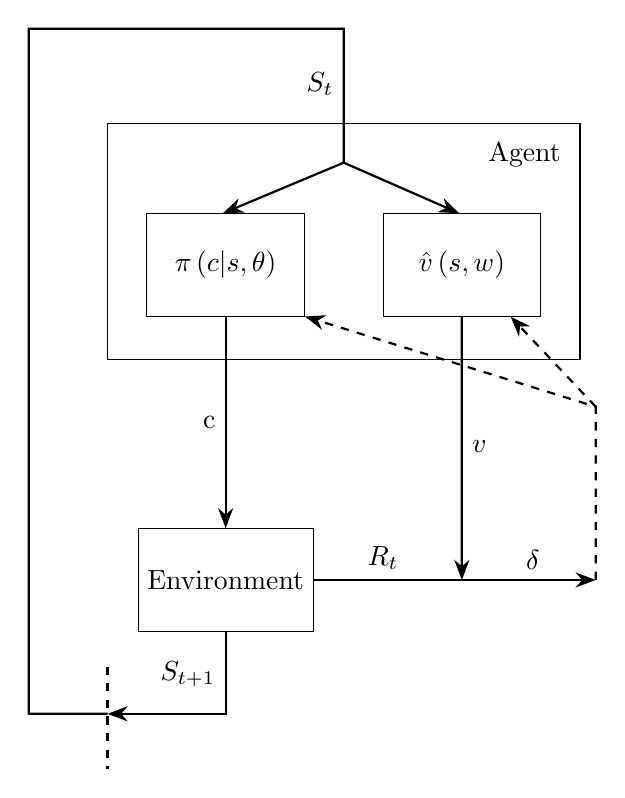
\begin{tikzpicture}[node distance=2cm]
        \node (agent) [process, minimum width=6cm, minimum height=3cm,
            label={[anchor=north east,inner sep=7pt]north east:Agent}]{};
        \node (pi) [process, left of=agent, xshift=0.5cm, yshift=-0.3cm]
            {\(\pi\left(c\middle|s,\bm{\theta}\right)\)};
        \node (v) [process, right of=pi, xshift=1cm]
            {\(\hat{v}\left(s,\bm{w}\right)\)};
        \node (env) [process, below of=pi, yshift=-2cm] {Environment};

        \draw [arrow] (pi) -- node[anchor=east] {c} (env);
        \draw [arrow] (env)
            -- ++(0,-1.7) node[anchor=east, yshift=0.5cm] {\(S_{t+1}\)}
            -- ++(-1.5,0) coordinate(next_s);
        \draw [arrow] (next_s) -- ++(-1,0) -- ++ (0,8.7) -- ++(4,0)
            -- ++(0,-1.7)
            node[anchor=east, yshift=1cm] {\(S_t\)} coordinate(m1)
            -- (pi.93);
        \draw [arrow] (m1) -- (v.93);
        \draw [arrow] (env)
            -- ++(3,0) coordinate(m2) node[anchor=south, xshift=-1cm] {\(R_t\)}
            -- +(1.7,0)
            node[anchor=south, xshift=-0.8cm] {\(\delta\)} coordinate(m3);
        \draw [arrow] (v) -- (m2) node[anchor=west, yshift=1.7cm] {\(v\)};
        \draw [dashed,arrow] (m3) -- ++(0,2.2) coordinate(m4) -- (pi.327);
        \draw [dashed,arrow] (m4) -- (v);
        \draw [dashed, thick] (-3,-5.4) -- (-3,-6.7);
    \end{tikzpicture}
    \caption{Actor-Critic for Finance Algorithm Illustration}
    \label{fig:a2c-illustration}
\end{figure}

\subsection{Training Result}
\noindent Figure~\ref{fig:a2c-out} shows the training result of 
Algorithm~\ref{algorithm:actor-critic} (300 moving average reward vs 
iteration), with 600 iterations (5 episodes per iteration), \(T=300\), 
\(\gamma=0.99\), \(\alpha_\theta=\alpha_{\bm{w}}=\num{3e-4}\).
\begin{figure*}
    \centering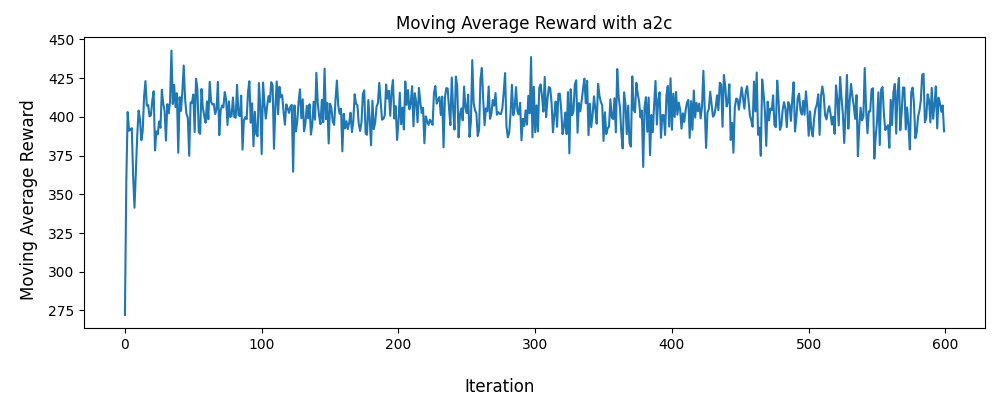
\includegraphics[scale=0.75]{a2c_out}
    \caption{Training Result for Algorithm a2c}
    \label{fig:a2c-out}
\end{figure*}
The graph shows that the moving average reward converges within only 50
iterations, that is, 250 episode, 75000 parameter updates for each network,
and stays quite stable afterwards.

\section{Actor-Critic, Reinforce, and PPO}
\subsection{Algorithms}
\noindent To further show how Actor-Critic algorithm performs, we compare it 
to another two popular algorithms: Reinforce 
(Algorithm~\ref{algorithm:reinforce}) and PPO (Algorithm~\ref{algorithm:ppo}).
\begin{algorithm}
    \caption{Reinforce for financial problem}\label{algorithm:reinforce}
    \begin{algorithmic}[1]
        \State Initialize ANN policy parameterization
        \(\pi\left(c\middle|s, \bm{\theta}\right)\), with any \(\bm{\theta}\)
        \State Step sizes \(\alpha_{\bm{\theta}}>0\)
        \Loop \hspace{0.3mm} (for each episode)
        \State Reset the environment
        \State Generate an episode 
        \(S_0, C_0, R_1, ..., S_{T-1}, C_{T-1}, R_T\),
        following \(\pi\left(\cdot\middle|\cdot, \bm{\theta}\right)\)
        \For{\(t=0, 1, ..., T\)}
        \State \(G \gets \sum_{k=t+1}^{T} \gamma^{k-t-1}R_k\)
        \State \(\bm{\theta} \gets \bm{\theta} + \alpha_{\bm{\theta}}\gamma^t
        G\nabla{\ln{\pi\left(C_t\middle|S_t, \bm{\theta}\right)}}\)
        \EndFor
        \EndLoop
    \end{algorithmic}
\end{algorithm}

\begin{algorithm*}
    \caption{PPO for financial problem}\label{algorithm:ppo}
    \begin{algorithmic}[1]
        \State Initialize ANN policy parameterization
        \(\pi\left(c\middle|s, \bm{\theta}\right)\), with any \(\bm{\theta}\)
        \State Initialize ANN state-value function parameterization
        \(\hat{v}(s,\bm{w})\) with any \(\bm{w}\).
        \State Step sizes \(\alpha_{\bm{\theta}}>0\), \(\alpha_{\bm{w}}>0\)
        \For{iteration \(k=0, 1, 2, ...\)}
        \State Collect set of trajectories \(\mathcal{D}_k=\{\tau_i\}\),
        following \(\pi\left(\cdot\middle|\cdot, \bm{\theta}_k\right)\), where
        \(\tau = S_0, C_0, R_1, ..., S_{T-1}, C_{T-1}, R_T\)
        \For{\(t=0, 1, ..., T\) in each trajectory \(\tau\) in 
        \(\mathcal{D}_k\)}
        \State \(G_t \gets \sum_{k=t+1}^{T} \gamma^{k-t-1}R_k\)
        \State \(A_t \gets G_t - \hat{v}(S_t)\)
        \EndFor
        \Loop \hspace{0.3mm} (update multiple times)
        \State \(\bm{\theta} \gets \underset{\bm{\theta}}{\text{arg\:max}}
        \frac{1}{|\mathcal{D}_k|T}
        \sum_{\tau\in\mathcal{D}_k}^{} \sum_{t=0}^{T}
        \min{\left(
                \frac{\pi\left(c_t\middle|S_t, \bm{\theta}\right)}
                {\pi\left(c_t\middle|S_t, \bm{\theta}_k\right)}A_t,
                \text{clip}\left(
                    \frac{\pi\left(c_t\middle|S_t, \bm{\theta}\right)}
                    {\pi\left(c_t\middle|S_t, \bm{\theta}_k\right)},
                    1-\epsilon, 1+\epsilon
                \right)A_t
        \right)}\)
        \State \(\bm{w} \gets \underset{\bm{w}}{\text{arg\:min}}
        \frac{1}{|\mathcal{D}_k|T}\sum_{\tau\in\mathcal{D}_k}^{} \sum_{t=0}^{T}
        \Bigl(\hat{v}(S_t, \bm{w})-G_t\Bigr)^2\)
        \EndLoop
        \EndFor
    \end{algorithmic}
\end{algorithm*}

\subsection{Training result}
\noindent To make better comparison, the policy function of the two algorithms
is implemented the same way as we did in Actor-Critic algorithm, and the same
is true for the value function used in PPO method.
\vspace{3mm}\newline Figure~\ref{fig:3-algorithms-out} shows the training 
result of these three algorithms (300 moving average reward vs iteration), 
with 600 iterations (5 episodes per iteration), \(T=300\), \(\gamma=0.99\),
\(\alpha_\theta=\num{3e-4}\), \(\alpha_{\bm{w}}=\num{3e-10}\) (if applicable),
\(\epsilon=0.5\) (if applicable).
\begin{figure*}
    \centering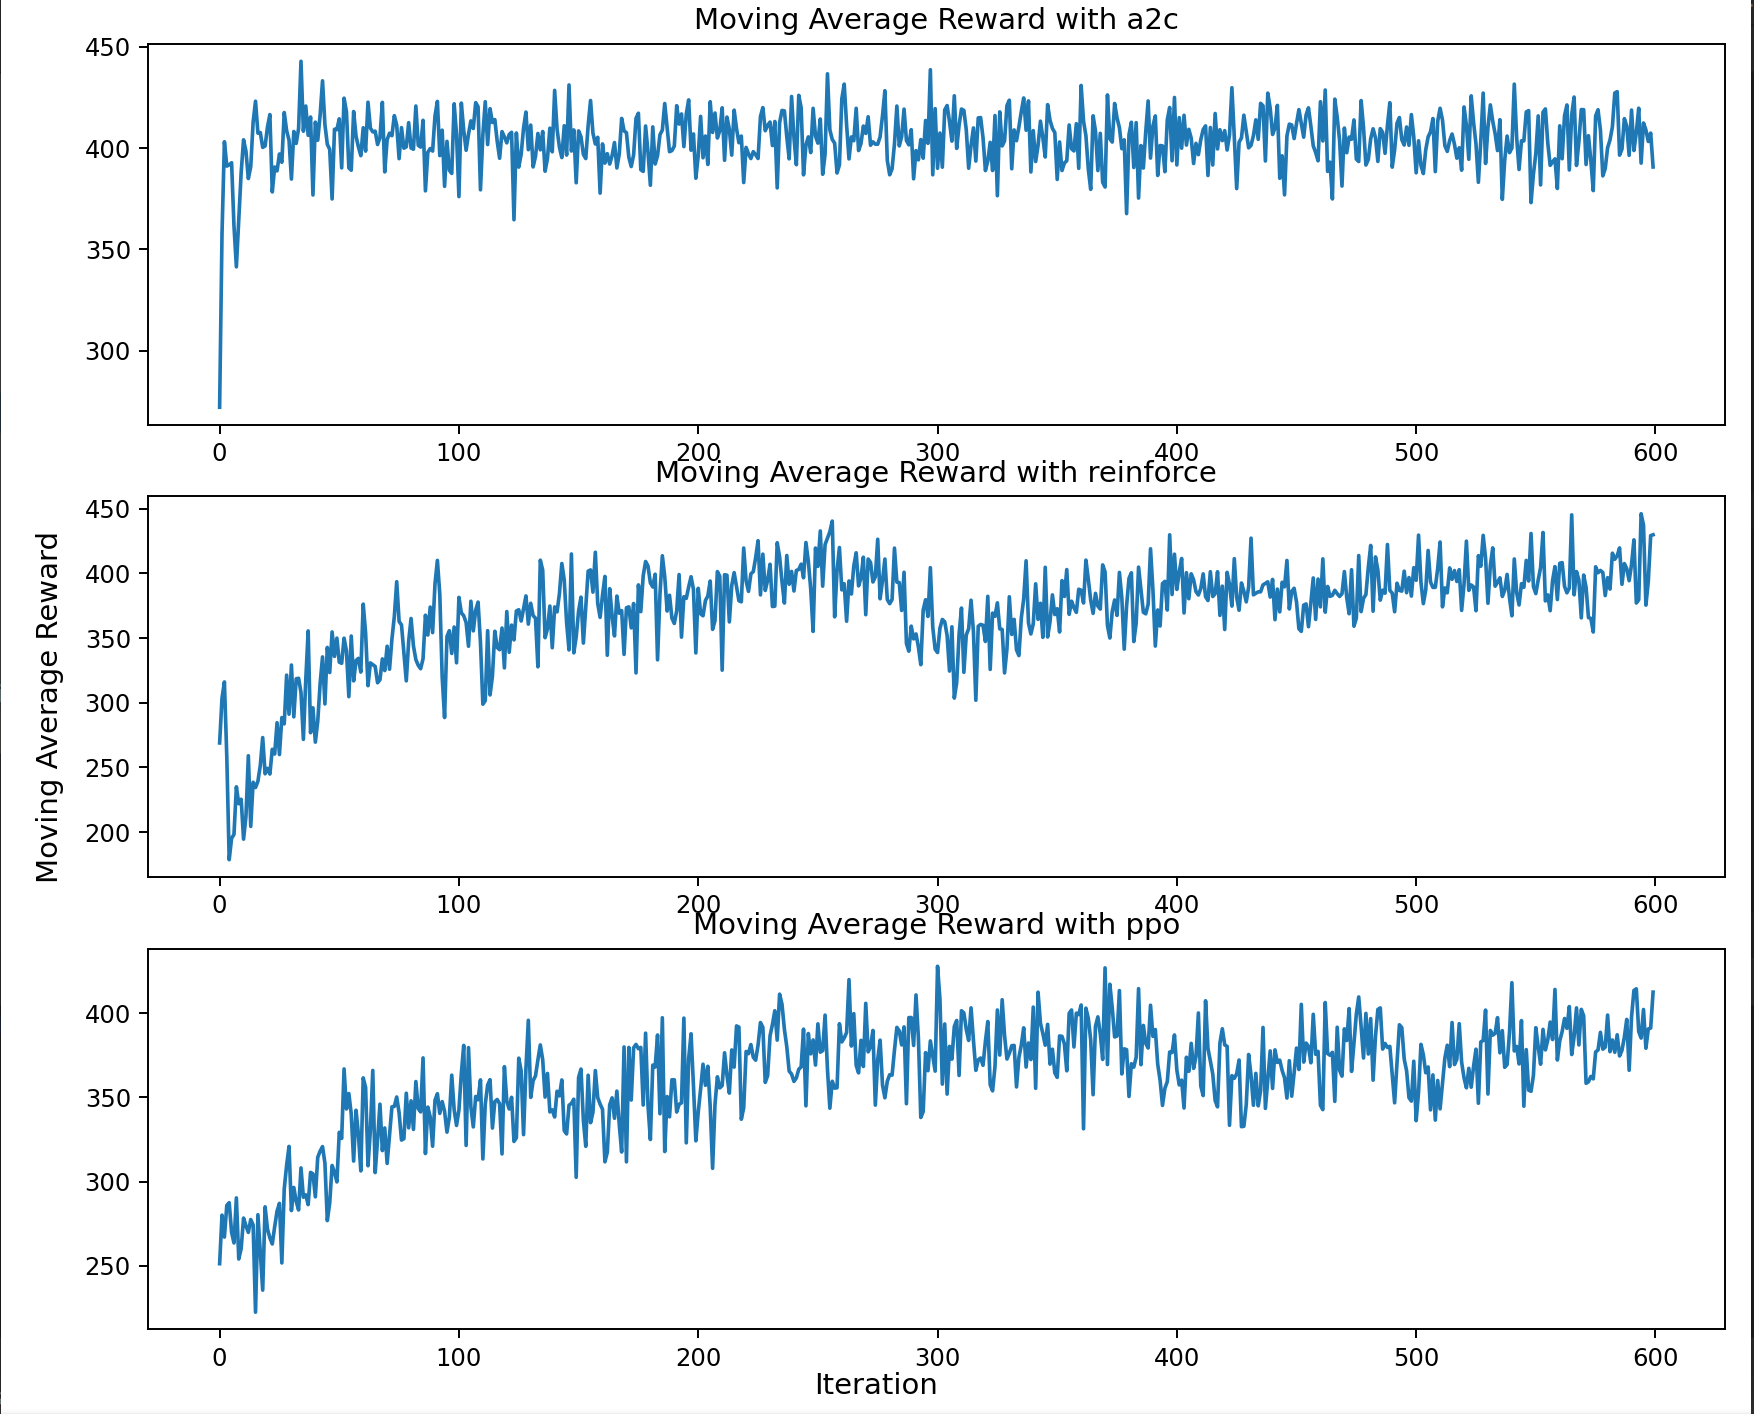
\includegraphics[scale=0.75]{out}
    \caption{Training Result Comparison for Three Algorithm}
    \label{fig:3-algorithms-out}
\end{figure*}
As is shown in Figure~\ref{fig:3-algorithms-out}, the Actor-Critic algorithm 
converges the fastest, within 50 iterations, followed by Reinforce algorithm, 
which converges within about 250 iterations, despite a small drop of moving 
average around iteration 300, which is quickly corrected by the algorithm 
within 50 iterations. PPO algorithm converges the slowest, with about 300 
iterations. Despite of the speed of convergence, the moving average rewards 
of convergence for these three algorithms are nearly the same (around 400), 
this is as expected.

\section{Conclusion}
\noindent Provide a brief conclusion (3-4 lines).

\section*{Acknowledgments}
\noindent Place any acknowledgments here.

%%%  REFERENCES  %%%%%%%%%%%%%%%%%%%%%%%%%%%%%%%%
%%
%% Put your references into your .bib file in the usual way. Run latex once, bibtex once, then latex twice.
%% The asmeconf.bst style allows @inproceedings and @proceedings to include: 
%%		venue = {Location of Conference}, 
%%		eventdate = {Month, days},

\nocite{*}%% <=== Delete this line unless you want to typeset the entire contents of your .bib file!

\bibliographystyle{asmeconf}  %% .bst file following ASME conference format. Do not change.
\bibliography{paper_2-col}

\end{document}

